% Chapter Template

\chapter{Introduction}

quick intro
\section{Background on biological patterning}
\subsection{Morphogenesis in nature, examples and function}
Periodic spatial structures in biology result from the emergent phenomena where a tissue of cells gains heterogeneity and complexity in the spatial domain following certain regularity/frequency.
These spatial structures can be widely observed in nature both in 2D such as the zebra's stripped skin or in 3D in the labyrinthian brain cortex.
Many other examples can be found in nature (See Figure ~\ref{fig:pattern_examples}).
Understanding the mechanism behind biological pattern formation is still a central question which remains elusive in the fields of systems, developmental and synthetic biology.  %todo comment on other applications
%they have also been used to gain insights into human settlement6 and to design water filters (Tan, Z., Chen, S., Peng, X., Zhang, L. & Gao, C. Science 360, 518–521 (2018).(Zincenko, A., Petrovskii, S., Volpert, V. & Banerjee, M. J. R. Soc. Interface 18, 20210034 (2021).). Experimentally, Turing patterns have been able to explain the spaced transverse ridges of the palate in mammals8. In 2021, researchers showed that a strained atomic bismuth monolayer on the surface of niobium diselenide displays Turing patterns9, an observation that may play a crucial part in the development of microdevices (Fuseya, Y. et al. Nat. Phys. 17, 1031–1036 (2021).).

\begin{figure}[h!]
    \centering
    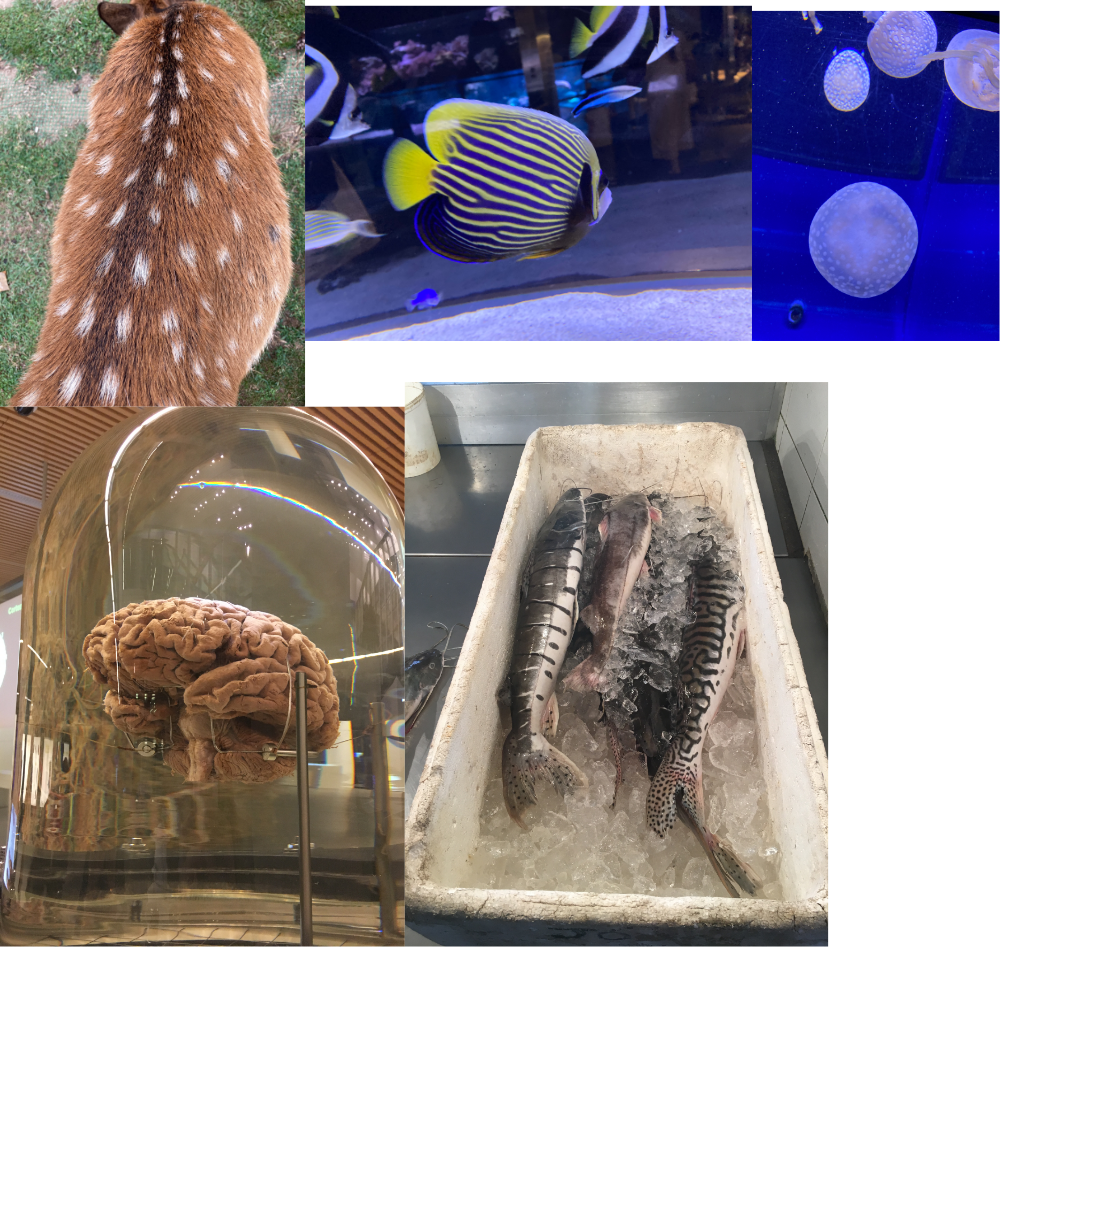
\includegraphics[width=1\textwidth]{chapters/Introduction/pattern_examples}
    \caption{\textbf{Title.} Caption}
    \label{fig:pattern_examples}
\end{figure}
%todo add all pattern images and the respective species if available
This evolution from simplicity to intricacy isn't merely aesthetic; it often plays a pivotal role in the functioning of multicellular beings.
Delving deeper, these patterns can have strategic advantages.
Fractal-shaped bacterial colonies, for instance, maximize nutrient absorption ~\parencite{Matsushita1990}.
Furthermore, distinct colorations, such as the zebra's stripes or the mesmerizing eye-spots on butterfly wings ~\parencite{Blest}, serve to disorient predators; either by disrupting the prey's silhouette or suggesting the prey is part of a larger entity ~\parencite{Stevens2006}.
The spirals observed in phylotaxis offer plants a way to optimize sunlight capture, enhancing photosynthesis ~\parencite{Strauss2020}.

The evolutionary advantage conveyed by this level of spatial organisation  hints towards genetic networks being potentially responsible for the patterning mechanism.
A randomly found solution of evolution where a pattern occurs, could lead to the genetic networks driving these spatial arrangements to be evolutionary beneficial and therefore selected.
Comprehending these networks and the dynamics that lead to these spatial designs is essential.
This area of research not only tries to understand which genetic networks and mechanisms are behind patterning, but also seeks to uncover how on a molecular scale these mechanisms are reliable, accurate and robust to the noisy and exposed biological environment.
Additionally, Studying this goes beyond understanding of developmental biology and morphogenesis.
It paves the way for pioneering work in biotechnological sectors, enabling the creation of intricately patterned tissues, efficient biofilms, or even organoids that hold potential in groundbreaking applications, such as tissue regeneration or organ implants ~\parencite{Scholes2017,Tan2018}. %todo comment on material deposition.



\subsection{Patterning theories}
Numerous mechanisms have been proposed in the literature to explain the formation in biological spatial systems.
Some of the most relevant ones can be categorized into mechanical instabilities and diffusion-based mechanisms %~\parencite{kosmrlj2020_2}.
The mechanical instabilities include phenomena such as differential adhesion, branching or wrinkling where physical forces are described in the model~\parencite{Scholes2017}.
% TODO SEARCH OTHER INSTABILITIES %todo cite other mechanical instabilities papers
On the other hand, gradient or diffusion based mechanisms rely on cells in the tissue responding to a molecule which is spatially heterogeneous and therefore exhibiting different phenotypes in different regions of the tissue (e.g.\ black vs white in zebra).


\section{Reaction-diffusion}
\subsection{Types of reaction diffusion: Wolpert vs Turing}
Among these gradient-based mechanisms, notable examples include positional information, the clock-and-wavefront model, and Turing instabilities ~\parencite{Wolpert1969, Baker2006, Turing1952}.
Both the positional information and clock-and-wavefront concepts are underpinned by an initial gradient of morphogens, interpreted by a genetic network to induce tissue patterns.
Sometimes, the origins of this gradient can be attributed to external factors such as ambient temperature, maternal impacts, or light exposure ~\parencite{Schier2009}.
However, in specific instances, the presence of an initial pre-pattern might be implausible, raising questions about how patterns spontaneously emerge from a prior uniform tissue.
Addressing this conundrum, the Turing's model offers an alternative as it doesn't need a pre-existing gradient and is self-organising ~\parencite{Kondo2010a}. %comment on space scaling, repetitive patterns and wide variety of shapes. check if the others can do it... i think not easily.
Given its attributes, the reaction-diffusion model might provide a more complete answer to the question of patterning in biology/ more holistic perspective on the intricacies of morphogenesis.
For this reason, Turing's mechanism for pattern formation will be the main focus of this work.
Nevertheless, it's pivotal to recognize that these mechanisms aren't strictly independent of each other.
The intricate nature of biological patterning might be best elucidated by an amalgamation of these theories, suggesting a blended framework may hold the answers ~\parencite{Green2015}. %todo discuss turings comment Turing himself recognized the biological unreality of this in stating that 'most of an organism, most of the time is developing from one pattern to another, rather than from homogeneity into a pattern' 1-34]
% TODO comment more on the fight between wolpert and turing and on the french flag model in general
\subsection{Turing patterns}
Reaction-diffusion systems were originally introduced in 1952 by Alan M. Turing in his paper “The chemical basis of morphogenesis” ~\parencite{Turing1952}.
In this article, he argues that pattern formation can be obtained when two morphogens interact with each other and diffuse at different
velocities across a tissue.
Morphogens, which are small molecules that can travel across the tissue and activate or inhibit other molecules.
If these morphogens are linked to growth hormones or skin pigments, biological patterns leading to a phenotype can arise.
The resulting patterns, called Turing patterns, can have different shapes such as stripes, labyrinths, spots; which can be widely observed in natural systems.
The concept of Turing patterns was first introduced from a mathematical perspective and was modelled using space and time dependent partial differential equations (PDE). In the case of Turing’s seminal paper, the set of PDEs describes a two node network (Fig.~\ref{fig:intro_to_turing_patterns}a) which has activation and inhibition terms, degradation terms and diffusion terms (Fig.~\ref{fig:intro_to_turing_patterns}b).
The key feature of this system is that it can exhibit diffusion driven instabilities: Initially, the tissue has a homogeneous concentration of morphogen under which no diffusion occurs, and under these circumstances the system is stable and converges into an equilibrium state.
When biological noise is introduced, the heterogeneity of the system leads to morphogen diffusion.
Consequently, the diffusion leads to changes in the reaction rates and the system is pushed out of steady state leading to an unstable system.
This unstable system converges into a stable stationary periodic pattern which is a Turing pattern (Fig.~\ref{fig:intro_to_turing_patterns}c).
This whole phenomena called the diffusion driven instability is the essence of Alan Turing’s paper and one of the most used mechanisms to explain morphogenesis.

\begin{figure}[h!]
    \centering
    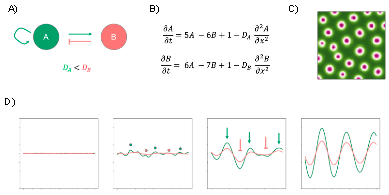
\includegraphics[width=1\textwidth]{chapters/Introduction/intro_to_turing_patterns}
    \caption{\textbf{Title.} Caption}
    \label{fig:intro_to_turing_patterns}
\end{figure}
%rerun simulations 2D, 1D snapshots and video


\subsection{Gierer Meindhardt}
Altough Turing’s work was of key importance in the field of developmental biology, it was not well accepted by biologists due to different reasons.
Firstly, the mathematical complexity behind it made it inaccessible for many scientists in the field.
Furthermore, the network proposed, although it can generate patterns, is too simple to describe the complexity in biological systems and takes some unrealistic assumptions such as the presence of negative concentrations ~\parencite{Kondo2010a}.
To solve these two issues, Gierer and Meindhardt proposed a generalised version of Turing’s diffusion-driven-instabilities ~\parencite{Gierer1972}.
This alternative theory proposes that patterns can be obtained as long as short-range activation and long-range inhibition (SALI) is present.
This implies that we can go away from Turing’s equations and extend the theory to networks with different number of nodes, different network interactions and even different signal transduction mechanisms ~\parencite{Murray1983, Rauch2004, Swindale1980}.
This step was necessary to be able to attribute patterning phenomena to more complex cellular and molecular interactions described by non-linear terms and larger networks with more nodes involved.
Examples of the first systems developed with non-linear terms are the typical Gierer-Meindhard model ~\parencite{Gierer1972}, Schnakenberg model ~\parencite{Schnakenberg1979}, as well as the Thomas model %~\parencite{thomas1976analysis}.
This generalisation work, sheds some light into the logic behind patterning and allows to understand it intuitively:
As an initially homogeneous system is perturbed by biological noise, local peaks of morphogen concentration form.
These transient peaks lead to a local activation effect where the concentration of all reactants increases.
Due to the difference in diffusivity, the inhibitor reaches further away and long range inhibition is achieved.
Ultimately, this system settles into a stationary pattern with activation peaks and inhibition troughs ~\parencite{Gierer1972}.
This SALI mechanism proposed by ~\cite{Gierer1972} can be better understood in Figure ~\ref{fig:intro_to_turing_patterns}d.
%todo maybe add more detail from detailed explanation: Imagine a system with two chemicals: an activator and an inhibitor. The activator stimulates its own production, that of the inhibitor, and the production of black pigment. The inhibitor, however, reduces the production of both activator and black pigment.This simple network leads to regular patterns when diffusion is introduced: these chemicals can spread, but they don't travel at the same speed. The activator moves slowly, affecting only nearby areas, while the inhibitor travels faster, reaching farther areas. As the activator starts working, a local region of black is produced. Some inhibitor is also produced, which travels faster than the activator, reaching further away and leading to inhibition and white in the areas surrounding the black. Once the inhibitor's effect diminishes in a distant region, the activator becomes dominant again, leading to another spot of pigment production. The repetition of this event across the tissue results in regular spots or stripes of pigment. These are the principles underpinning Alan Turing’s theory of pattern formation known as “Turing patterns”, which explain regular pattern formation in biology.

\subsection{Turing patterns in nature}
Various links have been made between biological patterns found in nature and Turing patterning networks.
As a basic example, seashell pigmentation and various types of fish skin have been replicated using simulations of Turing pattern systems.
Additionally, perturbation experiments in zebrafish’s skin are consistent with simulations of RD equations where the pattern regenerates in the exact same way after being physically disrupted both in-vivo and in-silico ~\parencite{Kondo2010a}.
Perturbation experiments are also carried out in the mammalian palatte, providing evidence of a Turing-type reaction-diffusion mechanism %todo cite palatte {economou}
Finally, molecules involved in patterning and morphogenesis have been shown to be part of networks with SALI characteristics.
For example, hair follicle development and fingerprint formation have been shown to rely on the same Turing reaction-diffusion network, based on signaling between EDAR, WNT, and antagonistic BMP pathways ~\parencite{Glover2023}
Other examples of Turing SALI networks are Nodal \& Lefty in right left assymetry ~\parencite{Nakamura2006}, Bmp \& Sox9 \& Wnt in limb digit development ~\parencite{J.Raspopovic1*L.Marcon1*L.Russo1J.Sharpe12014} and finally Wnt \& Dkk involve in lung branching ~\parencite{langhe2005_lung}.
All these examples of the relationship between biological patterns and RD systems, SALI networks and diffusion-driven instabilities strongly suggest that the Turing mechanism is linked to the self-assembling and self-regenerative patterns observed in nature.
However, the arguments mentioned above make Turing’s mechanism purely a strong hypothesis of patterning and do not prove causation.


%todo Feather patterning appears to similarly combine these mechanisms - reaction diffusino with cell movement (Ho et al.,2019).

%%todo add Recent experimental findings (Raspopovic et al., 2014; Junget al., 1998; Sick et al., 2006; Economou et al., 2012; Nakamasu et al., 2009) have resulted in Turing patterns being widely accepted as an important mechanism for spatial patterning in developmen-tal processes.

%
\section{Mathematical analysis of Turing patterns}

\subsection{Analysing Turing patterns}
Turing patterns are commonly studied using mathematical tools to understand their features and behaviours.
The equations describing these reaction-diffusion systems are usually too complex to solve analytically as they contain non-linearities and partial differential terms.
For this reason, different methods must be used such as linear stability analysis (LSA) or numerical methods.
LSA provides information on how the stability of the system evolves as we go from a system without diffusion to a system with diffusion ~\parencite{Glendinning1994}.
For RD systems to produce Turing patterns, they must be stable without diffusion and become unstable as diffusion is turned on ~\parencite{J.DMurray2002}.
This stability profile gives rise to the name “diffusion-driven instabilities” which is an alternative name to Turing patterns.
Overall, this method can tell us whether a system is a pattern generator, the wavelength and the relative speed of pattern formation.
Alternatively, numerical methods are used to calculate the concentration of species in the RD system at every time and space point ~\parencite{Ramos1983}.
A visual solution is obtained which provides information on the shape, wavelength, evolution and amplitude of the pattern.
While numerical methods provide more information than LSA, they are more computationally expensive and can lead to numerical errors ~\parencite{J.DMurray2002}.

In terms of the computational power and time required, recently developed tools such as VisualPDE can make it easier and faster to explore and get intuition on the numerical solutions a system ~\parencite{Walker2023}.
Both have their advantages or disadvantages and must be used in combination for an optimal study of RD systems and patterning.
\subsection{Fine-tuning problem}

Using both linear stability analysis and numerical methods, Turing patterns were widely studied to understand whether they were a plausible explanation for pattern formation in biology.
Although patterns were obtained analytically and numerically using models of the SALI networks mentioned above, the fine-tuning problem makes this mechanism questionable.
The fine-tuning problem or robustness problems refers to the small fraction of the parameter space leading to Turing patterns and high senstivity to parameter changes.
This issue was widely explored in ~\cite{Scholes2019}, where the parameter space of all 2-node and 3-node networks were studied using LSA to check for Turing patterning.
It was found that although 61\% of networks can produce Turing patterns, only 0.1\% of the parameter space is within Turing space.
Similar results were obtained in ~\cite{Zheng2016} and ~\cite{Marcon}.
To comment further into parameter tuning, original 2-node reaction diffusion systems require large differential diffusion rates between the two morphogens as explained previously for SALI mechanism to occur.
This is sometimes biologically unlikely, as many of the morphogens have similar diffusion rates due to their similarities in molecular size ~\parencite{huidobro}.
Finally, turing patterns can sometimes be sensitive to the initial conditions, leading to different patterns.
This is problematic as developmental biology expects robust patterns as cells need to respond to specific queus.   %todo find ref for this.

Another issue with Turing patterns is the sensitivity to the initial conditions.
Although the shape of the pattern is not strictly determined by the initial conditions, finer details like locations of spots and stripes can be influenced.
Additionally, although the final pattern is the same, the transient dynamics might differ between different initial conditions (e.g.\ different transient pattern or convergence time before settling into the final pattern). This can be an issue as in developmental biology, is a tighly controlled process where cells must receive the exact same signals in the same location and time in order to robustly reproduce the pattern. %todo find ref for this.





\subsection{Robustness of Turing patterns in realistic systems: bigger networks, growth, boundaries, noise, agar thickness}
On one hand, Turing's mechanism seems to explain many different patterns in biology as well as their perturbation experiments.
On the other hand, it does not seem a very robust mechanism.
How do these two contradicting ideas come together?
How can we make patterns more robust?
Typically, turing patterns are often studied in non-realistic systems.
A new direction in the field aims to study Turing patterns in more realistic systems large networks, systems with cooperativity, tissue discreteness at the cell level, growth, different boundary conditions, noise, delays, agar thickness. Surprisingly, some of these realistic biological conditions increase robustness for Turing pattern formation. %Studying Turing patterns with a more biological point of view can potentially help solve the robustness issue.

\subsubsection{Large networks}
Biological networks usually far from the idealised 2 node Turing networks. %todo quote average network size
Recent studies ~\parencite{Zheng2016, Scholes2019, Marcon} have shown larger networks exhibit greater robustness to parameter variations.
Specifically, it has been shown that adding an immobile substrate to a 2 node diffusible system relaxes differential diffusion constraints expected in the classic SALI topologies ~\parencite{korvasova2015}.
However, studying large networks is very computationally expensive because of various reasons including exponential increase in possible networks, increase in dimensions of the parameter space, increase in number of equations.
This has resulted in limited studies addressing larger networks than 3.
~\cite{Smith2018a} tackles this challenge by simplifying big networks into smaller ones.
The reduced model is not an accurate description of the original system.
However it can predict whether a system will not show instabilities, ruling out many cases to study and reducing the computational cost of exploring larger networks.
~\cite{Haas2021} studies large networks with 6 diffusers using a random matrix approach and also shows that there is a relaxation in differential diffusion constraints
This linearised random matrix approach previously used in ecology ~\parencite{May1972} could be used to explore large networks with mostly non-diffusible components that resemble the scale of real biological networks. %todo cite may without caps
%todo move somewhere else %Increase in robustness, and specifically decrease in differential diffusivity constraints is key to engineer biological pattern formation, as many available diffusers available in synthetic biology are predicted to diffuse at roughly equal speed due to their similarities in molecular weight ~\parencite{huidobro, Kondo2010a}

\subsubsection{High cooperativity}
Gene networks are usually described using non-linear Hill functions as many transcription factors exhibit allosteric behaviours in DNA binding. ~\parencite{Morgunova2017}
Greater cooperativity, reflected in steeper dose-response curves, can expand the Turing parameter space region and reduce the constraints imposed by differential diffusivity ~\parencite{Diambra2015a}.
%\subsubsection{Robust topologies}
%Studies have identified specific network topologies that exhibit enhanced robustness ~\parencite{Scholes2019}, which can be used when engineering patterns in synthetic biology. Nature probably converges into those topologies to maximise pattern formation robustness. The most robust topologies found in ~\cite{Scholes2019} are in line with the design principles found in other studies ~\parencite{Zheng2016} which show coherent activation and inhibition increases robustness.
%
%
%\item robust topologies and motifs: most robust topologies found in ~\parencite{Scholes2019}. This topology is in line with design principles
%found in other robustnes papaers try using as many AIJT topologies in the network as possible (coherent activation and inhibition) 2node core activation inhibition topology. ~\parencite{Zheng2016}. adding immobile no®de ~\parencite{Zheng2016,Diego2018} reduces need for differential diffusion.  %todo cite scholes most robust topology, msc thesis. %

\subsubsection{Discrete models}
Using discrete models can also show an increase in robustness.
Discretising concentration levels in ~\cite{Leyshon2021} which results in states rather than continuous kinetics, leads to some topologies being more robust to pattern formation. %todo justification of this discretisation.
Additionally, discretising space to cell size can lead to pattern formation in certain systems that usually do not allow it such as single diffuser networks ~\parencite{Wang2022}.

 % discrete models (discrete lattice gas cellular automaton (LGCA) framework.)concentration discreetenes: it confines the concentrations to a small number of discrete values (four in our case) and comprises discrete maps between these states rather than continuous kinetic parameters.Moreover, we found these five topologies to be more robust in the LGCA framework than they appear to be in the continuous case. ~\parencite{Leyshon2021}
 \subsubsection{Growth}
Fixed domains are often commonly assumed in developmental biology, as pattern forming processes (e.g reaction-diffusion of chemical species) occur at a much faster timescales than tissue growth. %todo add ref    %ref turing, ref 3 atlas papers
However, models of pattern formation in growing domains have shown growth to be extremely important in the development and morphology of the pattern.
Biological examples include angelfish \textit{Pomacanthus imperator} where growth induces the addition of new stripes in a branching point, while a constant wavelength ~\parencite{Kondo1995}.
In synthetic systems, the importance of growth can also be observed using a chemical reaction-diffusion system that grows over time ~\parencite{Konow2019}.
Slow growth rates were likely to produce rings that were added on the inside of the disk as it grew (inner ring addition), while fast growth rates produced rings on the outside (outer ring addition).
Intermediate growth rates formed labyrinthine structures.
All these principles of pattern morphology and growth rate are verified in the model.
These biological examples of growing patterns highlight the importance of including growth in models of pattern formation and specifically Turing patterns.

Considering the importance of growth in pattern morphology, it is key to consider how this growth might affect parametric robustness in Turing pattern formation.
Interesingly, introducing slow isotropic growth allows certain network topologies to form Turing patterns, which would not without growth.
An example of that are patterns in activator-activator networks, showing growth induced Turing instabilities.
Additionally, short-range activation and long-range inhibition can also produce Turing patterning in growing domains ~\cite{gaffney2010}.
Finally, increasing growth rates can increase the Turing parameter space under exponential growth in Turing patterning networks.
However, the analytical analysis used in ~\cite{gaffney2010} only holds when assuming slow isotropic growth and will break under faster growths.

Under logistic and linear growth, the Turing parameter space also changes.
However, the analysis used in ~\cite{gaffney2010} only holds when assuming slow isotropic growth and will break under faster growths.
This analysis is revisited in ~\cite{Klika2017} where they manage to study faster isotropic growing domains.
However, they observe that the conditions for Turing instabilities are more complex with higher growth rates and therefore more difficult to study than the ones in ~\cite{gaffney2010}.
This complexity makes it difficult to carry out high throughput studies of robustness and Turing parameter space in growing domains.
Finally, other types of growth such as anisotropic growth ~\parencite{Krause2019} are studied, but again they do not study parametric robustness in detail.

\subsubsection{Boundary conditions}.
Biological systems can exhibit a wide variety of boundary conditions depending on the context and environment.
Additionally, these boundary conditions can also be replicated using techniques in synthetic biology. (Krause et al.
2020b; Sheth et al.
2012; Vahey and Fletcher 2014; Dai et al.
2015).
Different theoretical studies explore a wide variety of boundary conditions for Turing systems.
Initially, it was shown that non-homogeneous boundary conditions where the system is not insulated, are less sensitive to changes in the domain size, different initial conditions and perturbations in model parameters ~\parencite{Arcuri1986}.
Then, mixed boundary conditions where different species are subject to different boundary definitions was also shown to increase parametric robustness ~\parencite{Maini1993, Maini1997, Krause2021}.
Studying these effects of these boundary conditions analytically is relatively complicated as you need to understand the bifurcation from which the Turing instability arises.
For example, although a Turing bifurcation is canonically a pitchfork bifurcation under Neumann boundary conditions, the Turing bifurcation is canonically a transcritical bifurcation under Dirichlet boundary conditions ~\parencite{Woolley2022}. %todo look at this again
This shows how much effect the boundaries have on the Turing instability, meaning they need to be considered when studying such systems.
An more applied biological example of how boundaries can affect pattern formation is seen in ~\parencite{Krause2020} where they study patterning synthetic biofilm in agar plates.
In this case, the agar absorbs the diffusers through the boundary, disrupting the pattern formed in the biofilm.
This effect can be reduced by decreasing the thickness of the agar layer.
Potentially, the pattern could also be maintained by reducing the permeability of the agar through the introduction of a filter paper or reduction of pore size.

%todo add robustness upon prepatternur

%
%Indeed, the idea that biological systems exchange material with their immediate environment seems likely in many situations. Therefore no-flux boundary conditions might be irrealistic.
%(point sources in butterfly wings %todo cite murray 1981)

%    also boundary between two different types of cells may give rise to morphogen production at the boundary interface %todo ~\parencite{meinhardt1981}.





\subsubsection{Noise}
Biological systems are known for their inherent noise.
In certain non-Turing parameter regimes, noise can drive diffusion-driven instabilities.
If there is a stable mode with eigenvalues slightly below zero, noise can destabilize this mode leading to a noise-induced instability and therefore the emergence of a pattern.
This might be a source of parametric robustness, producing patterns where deterministic systems do not predict one ~\parencite{Butler2009, Butler2011, Biancalani2010}.
Additionally, stochastic Turing patterns do not require large differential diffusivity between activator and inhibitor.
However, these patterns are not as ordered as deterministic Turing patterns ~\parencite{Karig2018}.
In terms of morphological robustness, deterministic Turing patterns were subjected to intrinsic noise using the same parameter region, and it was shown analytically that stochastically excited wave modes correspond exactly to their deterministic analogues, leading to a similar pattern.
Additionally, since noise perturbs populations away from the steady state, patterns can form quicker in a stochastic system than its deterministic counterpart ~\parencite{Maini2012}


\subsubsection{Delays} Having talked about realistic biological effects that contribute to pattern robustness, gene expression delays have been shown to do exactly the opposite.
Transcription and translation are biochemical processes that con occur in the scales of minutes to hours (depending on the size of the genomic sequence).
Therefore from a gene being activated to the protein being active there is a delay that is often not accounted when modelling patterning.
The pattern morphology has been shown to be extremely sensitive to delays including sensitivity to the initial conditions in the final pattern, dramatic changes in the patterning lag under different delays and even pattern loss when delays are introduced ~\parencite{Maini2012}.


Overall, it is important to understand how different phenomena can affect pattern formation and introduce in models the most relevant to the natural system or experimental system being studied.
Furthermore, in some cases, these biological phenomena could increase robustness to pattern formation and explain the lack of robustness found in classical Turing pattern studies ~\parencite{Scholes2019}.
%
%\item turing instability can appear through a pitchfork bifurcation (subcritical ) ---> l (Leppänen 2004; Benson et al. 1998;Crampin 2000;Dutt 2010, 2012; Grindrod 1996; Nicolis 1995; Auchmuty and Nicolis 1975; Bozzini et al. 2015; Breña-Medina and Champneys 2014; Dalwadi and Pearce 2022).  transcritical bifurcation
%Critically, the changes in bifurcation structure that are produced by altering the
%boundary conditions from Neumann to Dirichlet are not observed in the linear analy-
%sis,In this paper, we rectify this situation by demon-
%strating that although the Turing bifurcation is canonically a pitchfork bifurcation
%under Neumann boundary conditions (van Hecke et al. 1994), the Turing bifurcation
%is canonically a transcritical bifurcation under Dirichlet boundary conditions



\section{ Engineering reaction-diffusion patterns}
\subsection{previous attempts at engineering patterns}
As seen above, Turing patterns might benefit from realistic biological phenomena such as noise, boundary conditions ....
Engineering synthetic patterns could push all the theoretical knowledge on Turing patterns into a more applied field where these realistic biological conditions would be explored experimentally.
Furthermore, these synthetic patterns might benefit from the effects of these biological phenomena on robustness.

Although it is important to study patterning from a theoretical and mathematical point of view, it is also important to explore these systems experimentally.
As seen theoretically, many biological patterns that have been linked to Turing gene circuits %todo ref all the papers mentioned above on this.
However, due to the tangled nature of biological systems, it is extremely hard to prove that Turing’s mechanism is actually behind biological patterning.
Additionally, Turing patterns might benefit from realistic biological phenomena such as noise, boundary conditions ... etc.
Engineering synthetic patterns could push all the theoretical knowledge on Turing patterns into a more applied field where these realistic biological conditions would be explored experimentally.
Furthermore, these synthetic patterns might benefit from the effects of these biological phenomena on robustness.
For this reason, a bottom-up approach such as synthetic biology is required to understand if and how diffusion driven instabilities can lead to patterning in biology.
The aim of this bottom-up approach to build a system from first principles which is simpler, tunable and insulated from the tangled genetic context.
If this system is able to produce patterns, the mechanism is validated.
Furthermore, this synthetic system can be used to understand basic principles of developmental biology.
Additionally, synthetic patterning systems provide a powerful framework for tissue engineering ~\parencite{Scholes2017}. %todo comment on material deposition and other applications
The reason why we focus these engineering efforts in Turing patterns and not another mechanism is because they are extremely appealing for engineering as while having a simple network design, they exhibit unique self-organizing capabilities ~\parencite{Diambra2015a}.
However, before engineering Turing patterns, synthetic biology has had to slowly develop the tools by engineering simpler patterns.
In the field of synthetic biology, many simpler pattern generators have been engineered which range from systems without diffusers that rely on growth effects ~\parencite{Potvin-Trottier2016, Riglar2019}, to reaction diffusion systems relying on positional information ~\parencite{Barbier2020,Basu2005, Boehm2018, Grant2020, Kong2017, Schaerli2014}.
Some other engineered RD patterns do not rely on an initial gradient, however they are not able to form stationary periodic patterns ~\parencite{Cao2016, Danino2010, Payne2013}.
More detail on the existing synthetic patterning systems can be found in ~\parencite{huidobro}. %todo add more detail about this paper
%todo add paper review figure
All of these systems, although extremely interesting, cannot be classified as Turing patterns as none can self-assemble into stationary periodic patterns.
One of the closest attempts to synthetic Turing patterning is seen in ~\parencite{Karig2018} where stochastic Turing patterns are engineered using two orthogonal morphogens in E.coli. %todo solitons?
However, the patterns are not regular in wavelength, size and fluorescent intensity, which means they cannot explain the regular process of morphogenesis.
Alternatively, ~\cite{Sekine2018} uses an already existing patterning network (Nodal and lefty) in an eukaryotic system to produce self-assembling periodic patterns.
However, this type of pattern (called solitary localised structures) also varies in shape and size and is extremely sensitive to initial conditions.
Although elusive in synthetic biology, chemical Turing patterns have been successfully engineered in systems such as the chlorite-iodide-malonic acid (CIMA) reaction ~\parencite{Castets, Lengyel1992} or the thiourea-iodate-sulfite (TuIS) reaction ~\parencite{Horvath} where regular- repeat stationary Turing patterns can be observed.  %todo check these references against supermushroom and review paper
These are tunable systems which can be easily controlled (e.g with temperature), described with simple laws of mass action, have predictable parameters and are isolated from external components such as cell burden, or cross-talk ~\parencite{Butzin2018, Ceroni2015, Du2020, Nielsen2016}. %todo look at   Mu ̈ller et al 2019;
Although chemical systems have helped understand pattern formation and could prove key to tissue engineering applications, patterns in nature seem to go beyond just chemical patterns as they are closely linked to gene expression patterns as shown in \textit{in-situ} hybridization studies. %todo add cite [24–26]  , maybe is this   doi:10.1016/S0960-9822(02)01362-3,     doi:10.1016/j.mod.2006.03.006
For this reason, it is key to explore this avenue and build a genetically based Turing network that generates patterns in a biofilm.
The reason why we are interested in doing this with genes is because patterns in nature have been closely linked to gene expression as shown in in-situ hybridization studies





%todo comment that patterns are linked to gene expression because Modern experimental interrogations of suspected mor-phogen-based pattern formation systems, such as Nodal and Lefty zebrafish mesendodermal induction,use in situ hybridization [24–26]. This explicitly highlights local concentrations of specific mRNA tran- scripts and thus provides an indication of the rates of transcription of target genes, and emphasizes the role of gene expression in morphogenesis. Chen, Y. & Schier, A. F. 2002 Lefty proteins are long-
%range inhibitors of squint-mediated nodal signaling. Curr.
%Biol. 12, 2124–2128. (doi:10.1016/S0960-9822(02)01362-3)
%25 Jing, X. H., Zhou, S. M., Wang, W. Q. & Chen, Y. 2006
%Mechanisms underlying long- and short-range nodal
%signaling in Zebrafish. Mech. Dev. 123, 388–394.
%(doi:10.1016/j.mod.2006.03.006)
\subsection{engineering turing patterns in bacterial biofilms using exogenous circuit }
Even though they have been successfully engineered in chemical systems, the complexity of biology means that Turing patterns have never been engineered in a genetic context.
This can be attributed to the robustness problem including high sensitivity of parameters and a small fraction of parameter space producing Turing.
Additionally, designing Turing circuits with the classical 2 node topology leads to constrains in differential diffusivity that hinder the engineering of Turing patterns.
Finally, this fine-tuning issue is further amplified by the lack of orthogonal small-diffusible regulators to build a tunable synthetic pattering circuit.
All these issues have been addressed by previous researchers in the Isalan Lab and myself in order to achieve the engineering a synthetic circuit in bacteria that can produce Turing patterns.
Firstly, the ~\cite{Scholes2019} study found \("\)topology \(3954"\) which was amongst the most robust of the 3 node networks in terms of kinetic parameters.
Additionally, this topology allowed for equal diffusivity and even faster diffusing activators.
This discovery addresses partially the fine tuning problem and differential diffusivity constraints.
Then, new orthogonal diffusers were characterised in ~\cite{Meyer2019} and ~\cite{Du2020} which could be used to engineer the 3954 topology.
These toolboxes make it possible to bridge the gap between abstract models and real-sender receiver circuits.
Additionally, in ~\cite{huidobro} I compiled a list of small molecule regulators that can diffuse and form gene circuits in e.coli, as well as their respective promoters and synthesis enzymes.
Finally, ~\cite{Tica2020} engineered the 3954 topology using these components with the aim of exploring a robust Turing gene circuit for pattern formation.
Due to the lack of specific biological parts such as an inhibitor quorum sensing molecule or a dual inhibitor/activator molecule, the biological implementation of 3954 resulted in a 6 molecular specie circuit instead of the original 3 node network. %todo double check these are the constraints.
In this thesis, theoretical work was carried out relating to this gene circuit to understand how to tune parameters experimentally and what spatial setup to use to allow pattern formation in bacterial biofilms.
Furthermore, once patterns appear in the biofilm, to characterise and understand the mechanisms behind these patterns.
Having a genetic synthetic network that produces patterns with a predictive model would be is extremely impactful on various levels.
Firstly, the model would allow us to understand the patterning mechanisms behind the synthetic system and therefore shed some light into developmental biology.
Currently, our understanding is based on arbitrarily chosen models that match well the experiments, but that are not directly informed on well known and characterised gene circuits.
In this case we would have a model based on a known genetic circuit which matches the pattern generating experiments %todo comment on bespoke turing patterns
If this network can produce self-assembling periodic stationary patterns, it would prove that reaction-diffusion patterns can form in biological systems supported by genetic interactions.




%The issue of fine-tuning is further amplified by the lack of orthogonal small-diffusable regulators to build a tuneable synthetic pattering circuit.
%todo comment on bespoke turing patterns



%todo insert figure 2d

\section{project overview}
The aim of this thesis is to investigate Turing patterning in the context of synthetic biology and tissue engineering, using a modelling approach.
The first part of the thesis will take a more theoretical direction and do an in-depth investigation of how linear stability analysis relates to numerical solutions which themselves relate to the patterns seen in nature or experimentally .
This includes estimating wavelength, convergence time and in some cases pattern shape estimation from the dispersion relation.
Additionally, it also involves looking at which type of instabilities can produce stationary spatial patterns beyond Turing instabilities.
Going from this more theoretical approach, I will then consider realistic biological phenomena in the context of pattern formation such as different boundary conditions and growth.
Understanding how these phenomena affect pattern formation and its robustness, is key to understand which route to take when engineering pattern formation using synthetic gene circuits.
The second part of the thesis will focus on building a predictive model that can inform the experimental work in order to build a successful Turing pattern generator using gene circuits.
First, I will build a PDE system that describes the synthetic gene circuit engineered in ~\parencite{Tica2020}.
Then, I will explore the parameter space of this system to understand which regions are more robust in terms of pattern formation and how we can experimentally tune the genetic circuit in order to obtain a robust pattern generator.
Additionally, I will perform experiments where I grow small colonies with the synthetic gene network and image them using microscopy to observe fluorescence rings.
This experiment is continued by Jure Tica, Tong Zhu, Georg Wachter in larger colonies to observe a wide variety of patterns, including different types of stripes, spots and wedges.
Following this, I went on to develop a PDE solver combined with a cellular automata to model bacterial colony growth which I used to replicate all the patterns found.
Finally, the model is parametrised using minimisation and multivariate gaussian analysis, to constrain the parameters to more experimentally realistic values.
Inside the new parameter region, I find regimes which also produce Turing patterns, and more specifically the stationary rings observed.

%todo write one sentence summary of value of this thesis

